\section{Empirical and Engine Verification}\label{sec:eval}
We evaluate \system{} across two non-pooled layers: (i)~zero-LLM-call deterministic verification spanning finite authorization graphs, procedural Datalog closure scaling, seeded traceability, and headless Godot~4.7.1 soak tests, and (ii)~live neural suites pairing attested direct HTTPS Anthropic Claude~5.5 API protocols (\textbf{P15}--\textbf{P17}; $2.25\text{M}$ tokens across Haiku~5.5, Sonnet~5.5, and Opus~5.5 using \texttt{output\_config.json\_schema} with \texttt{temperature} omitted because Claude~5.5 rejects it as deprecated) alongside cross-family open/closed-weight CLI trials (\textbf{P11}--\textbf{P14}) retaining every failure in full denominators. Historical unexecuted cohorts (0/180 \texttt{20261103}; $N{=}0$ human \texttt{TR01--TR06}) remain isolated.

\subsection{Deterministic Boundary Audits, Godot Soak, and Datalog Scaling}\label{sec:kbs-det}
Across 1,664 finite-graph cases (416/arm$\times$4 plus 48 surface sentinels), \texttt{schema\_only} committed 260/416 invalid proposals, whereas every semantic-gate arm held \textbf{0/416} unsafe commits with 0/156 false rejections and 32/32 closure--BFS agreement; guided repair $\rho$ fixed 128/260 invalid candidates, lifting goal attainment from 124/416 to \textbf{252/416}. Extended zero-LLM checks confirm multi-error convergence (\textbf{A1}: 0/1,408 unsafe commits; 128/128 same-pass conflict freezes), sub-millisecond validator latency (\textbf{A2}: $N{=}2000$ p95 0.0042--0.0751\,ms; $R{=}256$ BFS/closure p95 0.312--0.478\,ms), seeded traceability (\textbf{A3}: 4,656/4,656 faults detected; 0/3,744 invariance false alarms), and headless Godot~4.7.1 engine soak stability (\textbf{A4}: 9/9 refusal codes exercised, 1,600/1,600 consistent ticks, \texttt{step\_commit} p95 0.708\,ms, $-268$\,B static delta; Fig.~\ref{fig:engine-cutscenes}). To verify assignment-complete denominator accounting before full live runs, we audited a 20-assignment v5 synthetic matrix (5 quest fixtures $\times$ 2 model selectors $\times$ Detailed/Generic feedback at $K{=}0$): 20/20 responses arrived, 10/20 passed strict schema parsing, 8/20 passed the semantic gate, and 7/20 reached the goal with zero unsafe mutations (Fig.~\ref{fig:paired-feedback-flow}). While 60 single-hop checks confirmed flat--ontology parity, five-world multi-hop closure (\textbf{P1}, 120 cases) and depth scaling (\textbf{P9}, 480 procedural cases across $R\in\{8,16,32,64\} \times d\in\{1..5\}$; Table~\ref{tab:kbs-det}) demonstrate that \texttt{nesy\_game.multihop} achieves \textbf{480/480 (100.0\% [99.21\%, 100.0\%])} bottom-up Datalog oracle parity at $O(d)$ $\le$7.12\,$\mu$s median latency, whereas 1-hop (46.67\%) and bounded 2-hop (60.00\%) fail at $d{\ge}2$ and $d{\ge}3$ ($Q{=}1100.19, p{=}6.88{\times}10^{-237}$).

\begin{figure*}[!tbp]
\centering
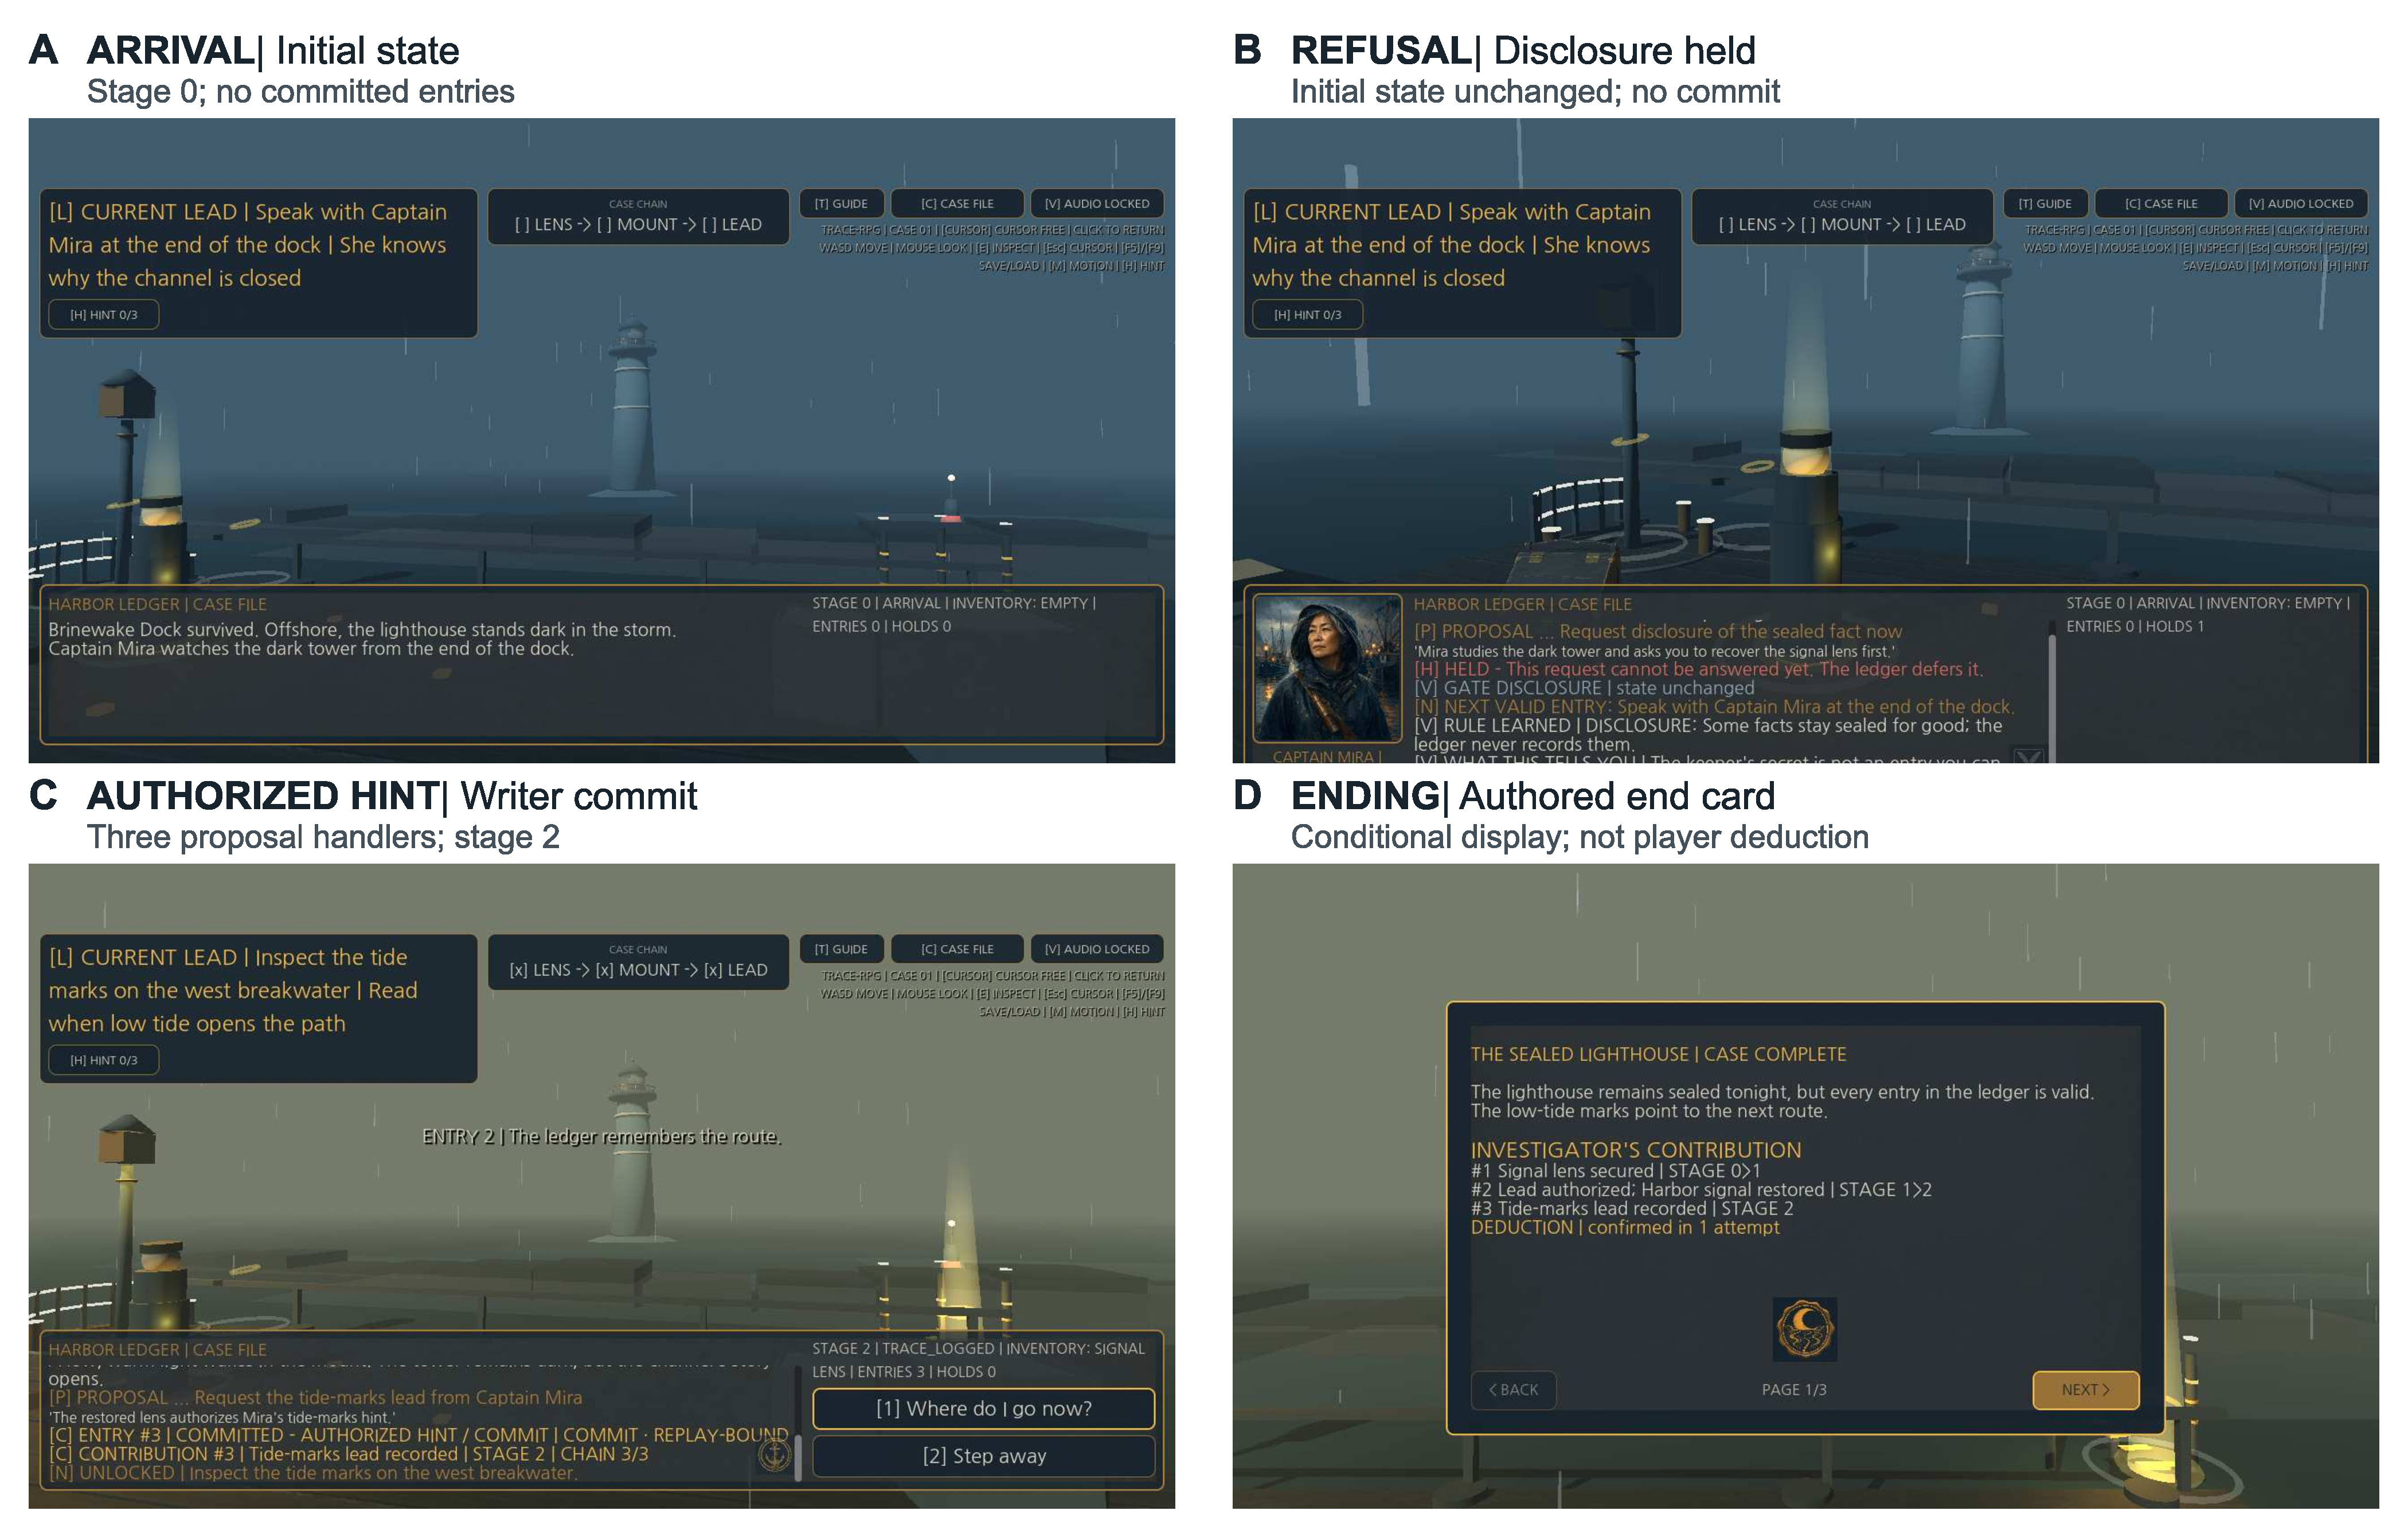
\includegraphics[width=0.90\textwidth]{../../figures/fig_engine_cutscenes.pdf}
\caption{Native Godot~4.7.1 engineering captures: (A)~initial arrival; (B)~denied premature secret disclosure with canonical state preserved; (C)~stage-2 authorized hint; (D)~conditional closing card.}
\Description{Four-panel Godot 4.7.1 screenshot sequence verifying engine state correspondence across arrival, denied disclosure, stage-2 hint, and closing card.}
\label{fig:engine-cutscenes}
\end{figure*}

\begin{figure}[!tbp]
\centering
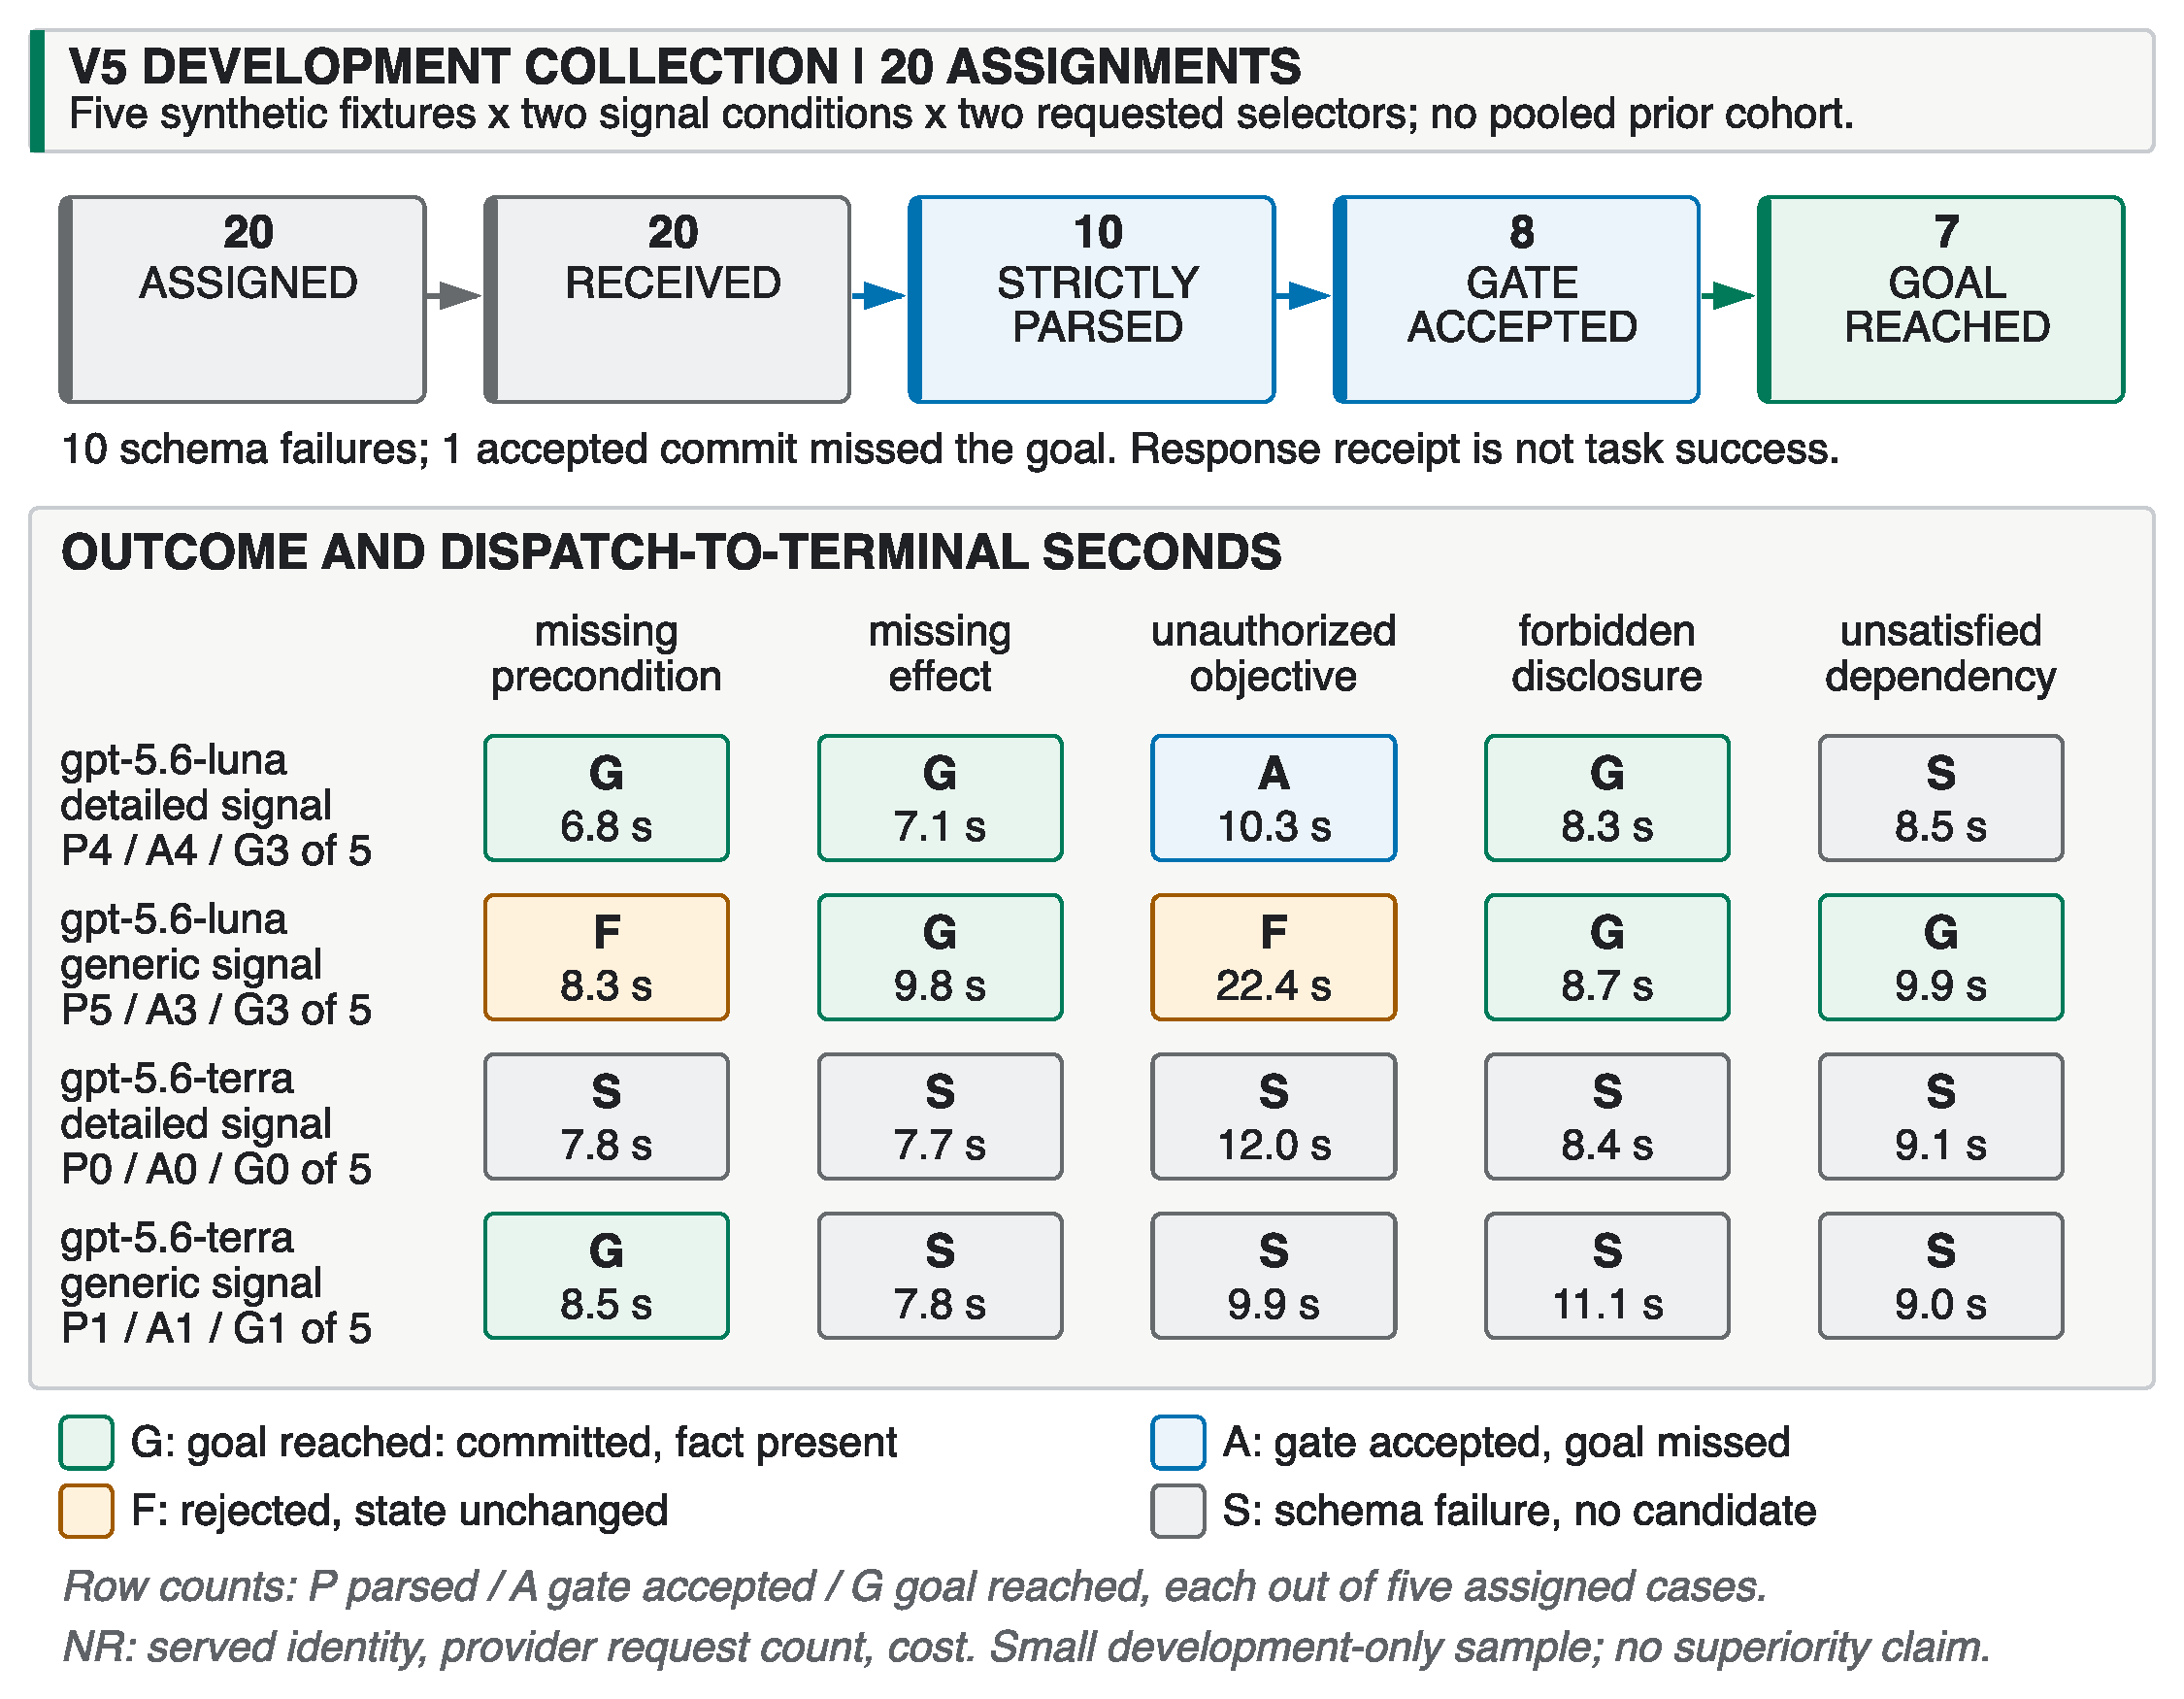
\includegraphics[width=\columnwidth]{../../figures/fig_paired_feedback_flow.pdf}
\caption{Assignment-complete flow on the 20-case synthetic collection: 10 schema failures remain in the denominator while 8 accepted candidates yield 7 goals.}
\Description{Sankey-style flow diagram across 20 assignments showing 10 parse failures, 8 gate passes, and 7 goal completions.}
\label{fig:paired-feedback-flow}
\end{figure}

\begin{table}[!tbp]
\caption{Zero-LLM Deterministic Boundary, Audit A1--A4, and Datalog Scaling (\textbf{P9}: 480 Procedural Cases)}
\label{tab:kbs-det}
\centering
\scriptsize
\setlength{\tabcolsep}{3pt}
\begin{tabularx}{\columnwidth}{@{}lcccc@{}}
\toprule
\textbf{Datalog Gate ($R{\le}64, d{\le}5$)} & \textbf{Acc.\ (480)} & \textbf{Leaks} & \textbf{Med.\ ($\mu$s)} & \textbf{p95 ($\mu$s)} \\
\midrule
\texttt{schema\_only} / \texttt{affordance} & 16.67\% (80) & 400 & --- & --- \\
\texttt{flat\_1hop\_gate} & 46.67\% (224) & 256 & 0.87--1.57 & 1.37--2.18 \\
\texttt{bounded\_2hop\_gate} & 60.00\% (288) & 192 & 1.88--2.58 & 2.66--3.91 \\
\texttt{nesy\_game.multihop} & \textbf{100.0\% (480)} & \textbf{0} & \textbf{6.46--7.12} & 9.83--11.42 \\
\bottomrule
\end{tabularx}
\end{table}

\subsection{Independent Closed-Loop 7-Arm Shielding and Cross-Family Negotiation (\textbf{P15} \& \textbf{P11})}
Table~\ref{tab:kbs-mas} reports \textbf{P15} (\textbf{105 independent 5-turn closed-loop trajectories} across Haiku, Sonnet, Opus~5.5 $\times$ 5 worlds $\times$ 7 arms; 1,048,803 tokens; \textbf{105/105} fresh 0-LLM replays exact) together with model-tier breakdowns. Controlled Safe-RL proxy masking~\cite{alshiekh2018shield} (0/15 safe goals, 1/15 zero-leak, 16/61 unsafe turns) and NeMo-style Colang proxy rails~\cite{rebedea2023nemo} (1/15, 1/15, 15/61) miss multi-hop derived and knowledge violations, and flat 1-hop gating still leaks 4/66 turns across 3/15 episodes in complex worlds (\texttt{ivory-citadel-v1}: 2 unsafe turns in 1/3 episode; \texttt{glass-foundry-v1}: 2 unsafe turns in 2/3 episodes). All three \texttt{nesy\_game.multihop} arms sustain \textbf{15/15 (100.0\% [79.61\%, 100.0\%])} zero-leak protection and \textbf{0} unsafe commits across all 3 tiers and all 5 worlds (3/3 per world). Crucially, every rejected candidate across \texttt{multihop\_k0} and \texttt{trace\_rpg\_multihop\_rho\_k2} in \textbf{P15} is a Theorem-2 state-dependent epistemic/stage violation, so $\rho$ maps all 18 blocked calls in \texttt{rho\_k2} to identity (\texttt{rho\_repairs=0}; the 14/15 [93.33\%] vs.\ 13/15 [86.67\%] difference over \texttt{k0} stems from independent Turn-1 LLM sampling on \texttt{haiku::ivory-citadel-v1}, not $\rho$ edits), whereas hybrid $\rho{+}\text{LLM}_{K=1}$ clears dead-ends via 20 Theorem-2 safe re-targets to reach \textbf{15/15 (100.0\%)} across Haiku, Sonnet, and Opus ($Q_{\mathrm{goal}}{=}68.714, p{=}7.50{\times}10^{-13}$; $Q_{\mathrm{zl}}{=}71.651, p{=}1.87{\times}10^{-13}$; McNemar vs.\ Safe-RL/NeMo $p{\le}1.22{\times}10^{-4}$). External 3-family CLI negotiation (\textbf{P11}: 30 episodes crossing Claude~Sonnet~5.5, open-weight GPT-OSS~120B, and Gemini~4~Hydrogen, 79/90 parsed, 11 GPT-OSS PF kept) confirms \textbf{30/30} zero-leak, 16/30 milestones, and \textbf{0/79} unsafe turns vs.\ Safe-RL (37/79, $p{=}9.5{\times}10^{-7}$), NeMo (43/79, $p{=}1.2{\times}10^{-7}$), and flat (29/79, $Q{=}118.93$).

\begin{table*}[!tbp]
\caption{Independent Closed-Loop 7-Arm Shielding with Exact Repair and Per-Tier Breakdown (\textbf{P15}: 105 Attested Episodes, 105/105 0-LLM Replays Valid)}
\label{tab:kbs-mas}
\centering
\scriptsize
\setlength{\tabcolsep}{3.0pt}
\begin{tabularx}{\textwidth}{@{}>{\raggedright\arraybackslash}Xcccccccc@{}}
\toprule
\textbf{Shielding Arm (15 ep/arm)} & \textbf{Safe Goal (95\% CI)} & \textbf{Zero-Leak} & \textbf{Unsafe} & \textbf{Blk/$\rho$/PF/Ret} & \textbf{Haiku} & \textbf{Sonnet} & \textbf{Opus} & \textbf{Tokens} \\
\midrule
\texttt{schema\_only} & 2/15 (13.3\%) [3.7, 37.9] & 2/15 & 16/59 & 0 / 0 / 0 / 0 & 1/1/6 & 1/1/4 & 0/0/6 & 133,054 \\
\texttt{safe\_rl\_action\_mask}~\cite{alshiekh2018shield} & 0/15 (0.0\%) [0.0, 20.4] & 1/15 & 16/61 & 2 / 0 / 0 / 0 & 0/1/5 & 0/0/5 & 0/0/6 & 139,205 \\
\texttt{nemo\_colang\_rail}~\cite{rebedea2023nemo} & 1/15 (6.7\%) [1.2, 29.8] & 1/15 & 15/61 & 1 / 0 / 1 / 0 & 0/0/5 & 0/0/5 & 1/1/5 & 136,515 \\
\texttt{flat\_1hop\_shield} & 12/15 (80.0\%) [54.8, 93.0] & 12/15 & 4/66 & 15 / 0 / 0 / 0 & 4/4/1 & 5/5/0 & 3/3/3 & 146,446 \\
\texttt{multihop\_shield\_k0} & 13/15 (86.7\%) [62.1, 96.3] & \textbf{15/15} & \textbf{0/69} & 22 / 0 / 0 / 0 & 4/5/0 & 5/5/0 & 4/5/0 & 152,649 \\
\texttt{trace\_rpg\_multihop\_rho\_k2} & 14/15 (93.3\%) [70.2, 98.8] & \textbf{15/15} & \textbf{0/68} & 18 / 0 / 0 / 0 & 5/5/0 & 5/5/0 & 4/5/0 & 150,986 \\
\texttt{trace\_rpg\_hybrid\_rho\_llm\_k1} & \textbf{15/15 (100\%)} [79.6, 100] & \textbf{15/15} & \textbf{0/63} & 2 / 0 / 1 / 20 & \textbf{5/5/0} & \textbf{5/5/0} & \textbf{5/5/0} & 189,948 \\
\bottomrule
\end{tabularx}
\end{table*}

\subsection{Attested Prospective Factorial Ablations (\textbf{P16A}) and Fair $(a,E)$ Repair (\textbf{P12})}
Table~\ref{tab:kbs-p16a} disaggregates all 60 prospective factorial episodes of \textbf{P16A} across representation, model tier, and quest world (673,869 tokens, non-pooled with frozen 0/180 \texttt{20261103}). Under \texttt{general\_rule}, Sonnet (4 unsafe commits) and Opus (5 unsafe commits) breach multi-hop knowledge/role checks in \texttt{ivory-citadel-v1} (4) and \texttt{glass-foundry-v1} (5), yielding 0/30 goals and 22/30 (73.33\%) zero-leak. Switching to \texttt{ontology\_multihop} enforces \textbf{30/30 (100.0\%)} zero-leak (McNemar $p{=}0.00781$), \textbf{0} unsafe commits across every tier and world, 22 runtime repairs (Haiku 18, Sonnet 4), and \textbf{11/30 (36.67\%)} safe goals (Opus 8/10, Sonnet 3/10, Haiku 0/10; $p{=}9.77{\times}10^{-4}$). Complementing this factorial test, \textbf{P12} (90 5-world proposals, 84/90 parsed) confirms \textbf{0/84} unsafe commits only under \system{} vs.\ Safe-RL (54/84), NeMo (55/84), and flat 1-hop (32/84; $Q{=}281.23$); on 27 matched policy+stage faults given equal $(a,E)$ counterexamples, deterministic $\rho_{K=2}$ hits \textbf{27/27 (100.0\%)} at 0 extra tokens vs.\ matched State-Blind and State-Aware LLM $K{=}2$ (both 26/27 = 96.3\% at 530,044--542,042 extra tokens / $>$508\,s, $p{=}1.0$), isolating zero-token latency elimination and Theorem~2 non-laundering fallback.

\begin{table}[!tbp]
\caption{Per-Tier and Per-World Disaggregation in Attested Factorial Suite (\textbf{P16A}: 60 Episodes; \texttt{gen}/\texttt{ont} = \texttt{general\_rule}/\texttt{ontology\_multihop})}
\label{tab:kbs-p16a}
\centering
\scriptsize
\setlength{\tabcolsep}{1.5pt}
\begin{tabularx}{\columnwidth}{@{}>{\raggedright\arraybackslash}X*{6}{c}@{}}
\toprule
\textbf{Stratum} & \textbf{Goal (\texttt{g/o})} & \textbf{Zero-Leak} & \textbf{Unsf.} & \textbf{Rep.} & \textbf{PF} & \textbf{Tok (k)} \\
\midrule
Overall (30/30) & 0/30 / \textbf{11/30} & 22/30 / \textbf{30/30} & 9/\textbf{0} & 0/22 & 1/1 & 294/380 \\
\texttt{claude-haiku} & 0/10 / 0/10 & 10/10 / 10/10 & 0/0 & 0/18 & 0/1 & 104/138 \\
\texttt{claude-sonnet} & 0/10 / 3/10 & 6/10 / \textbf{10/10} & 4/\textbf{0} & 0/4 & 0/0 & 104/130 \\
\texttt{claude-opus} & 0/10 / \textbf{8/10} & 6/10 / \textbf{10/10} & 5/\textbf{0} & 0/0 & 1/0 & 85/112 \\
\midrule
\texttt{lighthouse} & 0/6 / 2/6 & 6/6 / 6/6 & 0/0 & 0/6 & 0/1 & 59/75 \\
\texttt{archive} & 0/6 / 0/6 & 6/6 / 6/6 & 0/0 & 0/8 & 0/0 & 60/79 \\
\texttt{observatory} & 0/6 / 2/6 & 6/6 / 6/6 & 0/0 & 0/2 & 0/0 & 61/77 \\
\texttt{ivory-citadel} & 0/6 / 3/6 & 2/6 / \textbf{6/6} & 4/\textbf{0} & 0/4 & 1/0 & 58/79 \\
\texttt{glass-foundry} & 0/6 / \textbf{4/6} & 2/6 / \textbf{6/6} & 5/\textbf{0} & 0/2 & 0/0 & 55/70 \\
\bottomrule
\end{tabularx}
\end{table}

\subsection{Headless Godot~4.7.1 Engine Execution (\textbf{P16B} \& \textbf{P13})}
In attested live Godot~4.7.1 execution (\textbf{P16B}: 21 closed-loop episodes across Haiku, Sonnet, Opus~5.5, 169,071 tokens), every trajectory re-executes inside headless Godot~4.7.1 (\texttt{4.7.1.\allowbreak stable.\allowbreak official.\allowbreak a13da4feb}) with 0 LLM calls at verification time: \textbf{21/21} fresh replays pass, \textbf{0/21} unsafe commits/leaks occur, \textbf{13/15} five-world goals succeed (Haiku 5/5, Sonnet 4/5, Opus 4/5; Godot runtime 251.64--1009.78\,ms vs.\ API 10,606--40,892\,ms), and \textbf{6/6 (100.0\%)} production \texttt{SealedLighthouseMachine} runs under both \texttt{standard} and \texttt{social\_pressure} regimes match \texttt{EXACT\_\allowbreak TERMINAL\_\allowbreak HASH} (\texttt{4b231017...}; Godot 751.30--778.80\,ms vs.\ API 9,055--16,485\,ms). This parallels 3-family CLI Godot~4.7.1 results (\textbf{P13}: 42/42 replays valid, 0/42 leaks, Claude \& Hydrogen 14/14 goals vs.\ GPT-OSS 4/14).

\subsection{Unified Stage-1 + Stage-2 Bilingual Escape (\textbf{P17} \& \textbf{P14})}
Table~\ref{tab:kbs-p17} details \textbf{P17}: \textbf{540} fresh API evaluations using one identical prompt across 180 EN/KO cases (90 EN, 90 KO; 3 domains $\times$ 60 cases; 0 deterministic short-circuits, 359,030 tokens; Fleiss' $\kappa{=}0.8813$, $\alpha{=}0.8815$, $Q{=}9.5, p{=}0.00865$). Every Claude~5.5 tier achieves \textbf{0/72 (0.0\%) FRR} and 94.44--97.22\% paraphrase recall (significantly outperforming calibrated rule hybrid on Haiku $p{=}1.12{\times}10^{-4}$ and Opus $p{=}0.00940$, with no language collapse across EN/KO). Yet neural tiers miss 7--17/36 unhinted explicit ID tokens inside neutral prose (especially \texttt{keeper\_secret}: Sonnet 2/12, Haiku/Opus 5/12), demonstrating why symbolic Stage-1 gating (36/36 explicit) and Stage-2 neural detection must operate jointly. Cross-family 720-eval checks (\textbf{P14}) corroborate open-weight parity (\texttt{gpt-oss-120b-medium} $F_1{=}0.9714$, $\kappa{=}0.9367$), and all Phase-1--5 artifacts are indexed under \texttt{DATASHEET\_v5.md}~\cite{gebru2021datasheets} and Croissant~1.0 v5~\cite{akhtar2024croissant} (26/26 SHA-256 digests).

\begin{table}[!tbp]
\caption{Unified-Prompt Bilingual Escape Disaggregation (\textbf{P17}: 180 EN/KO Cases $\times$ 3 Tiers = 540 Evals, 0 Short-Circuits)}
\label{tab:kbs-p17}
\centering
\scriptsize
\setlength{\tabcolsep}{1.4pt}
\begin{tabularx}{\columnwidth}{@{}>{\raggedright\arraybackslash}X*{6}{c}@{}}
\toprule
\textbf{Verifier} & \textbf{Exp} & \textbf{Para} & \textbf{FRR} & \textbf{$F_1$} & \textbf{EN/KO} & \textbf{Domains} \\
\midrule
\texttt{id\_only} & \textbf{36/36} & 0/72 & 0/72 & .500 & --- & .50/.50/.50 \\
\texttt{loo\_tfidf} & \textbf{36/36} & 45/72 & 45/72 & .692 & --- & .70/.66/.72 \\
\texttt{rule\_hybrid} & \textbf{36/36} & 38/72 & 0/72 & .813 & --- & .64/.94/.82 \\
\texttt{haiku-5-5} & 29/36 & \textbf{70/72} & \textbf{0/72} & \textbf{.957} & .95/.96 & .88/.99/\textbf{1.0} \\
\texttt{sonnet-5-5} & 19/36 & \textbf{70/72} & \textbf{0/72} & .904 & .92/.89 & .84/.89/.97 \\
\texttt{opus-5-5} & 25/36 & 68/72 & \textbf{0/72} & .925 & .94/.91 & .89/.89/.99 \\
\bottomrule
\end{tabularx}
\end{table}
